\chapter{Contexte général du projet}
	Cette partie traitera du contexte général de notre projet d’Innovation et de Conception, en mettant l’accent essentiellement sur une brève présentation du maître d'ouvrage et de ses exigences fonctionnelles. Également, la méthodologie de travail adoptée ainsi que la planification du projet seront mises en avant.  
	\newpage
	\section {Contexte général du projet}
	\subsection{La ligue des Hauts-de-France du triathlon }
	
	La Ligue des Hauts-de-France de Triathlon est un organe décentralisé de la F.F.TRI. Elle est administrée par un Comité Directeur et un Bureau Directeur composés de membres élus en son sein. 
	Pour fonctionner, la ligue Hauts-de-France, a constitué plusieurs commissions dont chacune est présidée par un membre du Comité Directeur et composées de membres de la ligue volontaires et choisis pour leurs compétences.
	Celle-ci n'a été créé que récemment, car elle fait suite à la fusion des régions Picardie et Nord-Pas-de-Calais.
	L'assemblée générale s'est alors tenu le 03 février 2018, \href{http://triathlonhdf.fr/samedi-03-fevrier-2018-la-ligue-des-hauts-de-france-de-triathlon-est-creee/}{un court article a été rédigée sur leur nouveau site web à l'adresse triathlonhdf.fr} \cite{ref1}
	
	\subsection{Description du processus de l’organisation des challenges }
	L’organisateur de la course envoie les informations de tous les participants ainsi que leurs classements à la ligue. Ces fichiers sont envoyés sous formats PDF, Word, Tableurs Excel voire même papier.  Ces données sont envoyées à la ligue sans aucun traitement ou filtrage. Par conséquent, les administrateurs de la ligue ont pour première tâche de supprimer les participants qui ne sont pas inscrits au niveau de la ligue, et également de traiter le problème des homonymes d’une manière manuelle. Tâche qui demeure difficile et demande du temps.
	Une fois les données sont actualisées, les fichiers challenge sont mis à jour et les classements globaux sont établis. L’ensemble de ces opérations sont faites moyennant des fichiers Excel.
	
	
	\subsection{Les modalités du challenge  }
	Les challenges organisés sont soumis à plusieurs règles qui sont répertoriées comme suit :
	\begin{itemize} 
	\item 	Toutes les épreuves individuelles de cross duathlon, duathlon, aquathlon, cross triathlon et triathlon organisées par la Ligue NPdC, distance XS, S, M, L ou XL sont retenues pour le challenge.
	\item 	Les organisations s'inscrivant dans le circuit des épreuves du challenge doivent se soumettre au cahier des charges proposés par la Ligue.
	 \item  Seront retenues au challenge de l’année suivante uniquement les épreuves qui rempliront les contraintes et fourniront les résultats au format prévu au point 8 au plus tard dans la semaine suivant l’épreuve.
	
	\end{itemize} 
\newpage
	 Attribution des points. Un classement individuel par catégorie et par sexe est réalisé à l’issue de chacune des épreuves. Seule la distance la plus longue accessible à la catégorie sera prise en compte dans l’obtention des points.\\
	L’attribution des points se fait en fonction du classement par catégorie et sexe. 
	
	Les tableaux figurant ci-dessous récapitulent le nombre de points attribués selon le classement du participant :
	\begin{enumerate}
	   \item Pour les adultes
	\begin{figure}[h!]
	   \center
	   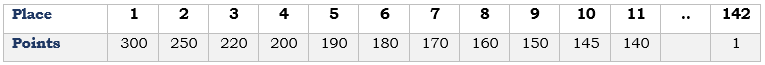
\includegraphics[scale=1]{img/points_categorie_adultes.png}
	   \caption {Les points attribués aux participants de la catégorie adultes selon leurs classements}
	\end{figure}
	
	Au-delà de la 142ème place, 1 point est attribué à chacun des participants. Les points obtenus sont pondérés par un coefficient dépendant de la distance de l’épreuve : 
	
	\begin{itemize} 
	 	\item 0,5 pour un XS ; 
	 	\item 0,75 pour un S ;
	 	\item 1 pour un M ; 
	 	\item 1,5 pour un L ;
	 	\item 2 pour un XL ou XXL.
	\end{itemize} 
	   \item Pour les jeunes
	\begin{figure}[!h]
	   \center
	   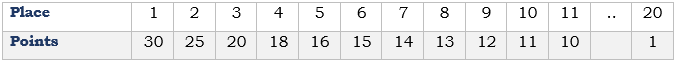
\includegraphics[scale=0.9]{img/points_categorie_jeunes.png}
	   \caption {Les points attribués aux participants de la catégorie jeunes selon leurs classements}
	\end{figure}
	
	\end{enumerate}

	\newpage
	Au-delà de la 20ème place, un point est attribué à chacun des participants. Les abandons et les absents ne marquent pas de point. 
	L’ensemble des règles susmentionnées sont récapitulées dans le schéma suivant :
	\begin{figure}[!h]
	   \center
	   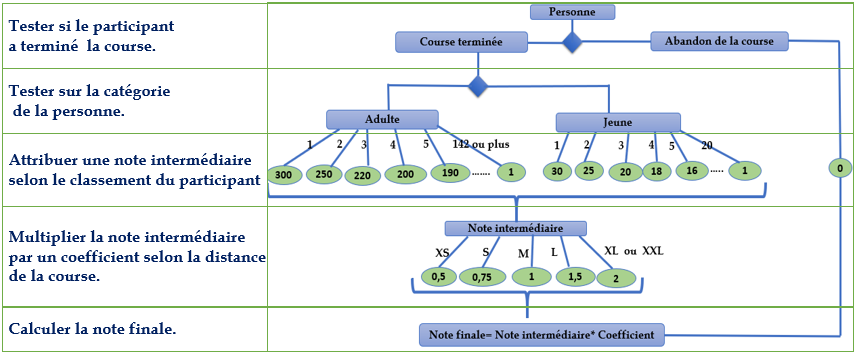
\includegraphics[scale=0.9]{img/recapitulatif_modalite_challenge.png}
	   \caption {Récapitulatif des modalités du challenge}
	\end{figure}
	
	\newpage
	\subsection{Expression des besoins fonctionnelles}
	L’outil développé dans le cadre de ce projet, doit répondre aux fonctionnalités définies en concertation avec le client lors des réunions. Ainsi l’ensemble de ces fonctionnalités sont répertoriées comme suit :
	\begin{itemize} 
	\item Supprimer les participants dans une courses et qui ne sont pas inscrits dans la ligue ;	
	\item Pallier au problème des homonymes ;
	\item Création d’un challenge
	\item La mise à jour d’un challenge ;
	\item Affichage des résultats globaux des courses ;
	\item Afficher les statiques individuels avec les graphes correspondants ;
	\item Effectuer des recherches des participants par plusieurs critères ;
	\item Toutes ces opérations doivent être réalisées émanant une interface graphique reluisante.
	\end{itemize} 
	
	\subsection {Méthodologie de travail }
	Afin de garantir la réussite du projet, il a été décidé de recourir à la méthodes agile SCRUM. En effet, celle-ci consiste à découper le projet en boites de temps appelées sprints. Chaque sprint commence par une estimation suivie d'une planification opérationnelle. Le sprint se termine par une démonstration de ce qui a été achevé. Avant de démarrer un nouveau sprint, l'équipe réalise une rétrospective. Cette technique analyse le déroulement du sprint achevé, afin d'améliorer ses pratiques. Le flot de travail de l'équipe de développement est facilité par son auto-organisation. 
	Pour mettre cette méthode en pratique. Une réunion est organisée chaque jeudi après-midi avec nos Encadrants pour discuter des avancements de la semaine en cours en de déterminer les tâches à effectuer durant la semaine à avenir. Par ailleurs, l’ensemble des tâches à réaliser sont répartis sur les membres de l’équipe afin de converger les efforts pour la réussite du projet. 
	
	
	\subsection{Diagramme de Gantt}
	La planification est parmi les phases d’avant-projet. Elle consiste à prévoir le déroulement du projet tout au long de ses phases. Grâce aux réunions tenues avec nos encadrants et le client, on a été éclairés sur les différentes étapes du projet.
	Ainsi le diagramme ci-après résume les différentes étapes ainsi que le temps qui leurs a été allouée
	\begin{figure}[!h]
	   \center
	   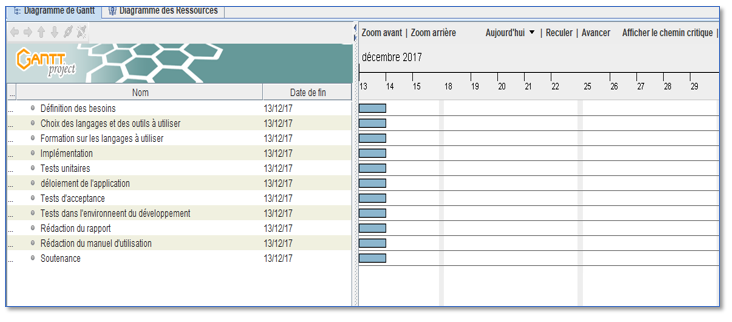
\includegraphics[scale=0.9]{img/diagramme_Gantt.png}
	   \caption {Le diagramme de Gantt du projet}
	\end{figure}
	\newpage
	
